\chapter{Revisão Bibliográfica} \label{cap2}
\section{Fundamentação Teórica}
\subsection{Redes Neurais}
Redes neurais são modelos computacionais inspirados no sistema nervoso humano. Suas estruturas são subdivididas em camadas e unidades de processamento. As camadas representam a ordem nas quais os neurônios processam as informações. Os neurônios são as unidades de processamento, onde similarmente ao sistema nervoso, recebem um estimulo, processam e transmitem o estimulo aos demais neurônios da rede neural. A estrutura de um neurônio pode ser vista na figura a seguir:
\begin{figure}[h]
	\centering
    \label{fig1}
    \vspace{3ex}%
	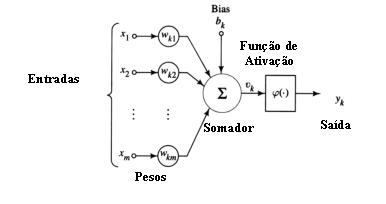
\includegraphics[scale=0.7]{pasta1_figuras/neuronio_artificial.jpg}
    \caption{Neurônio Artificial}
\end{figure}

Como nos neurônios presentes no sistema nervoso, o neorônio artificial possui um meio de recepção dos estimulos vindos do meio externo, que são denominadas as entradas. Os pesos são atribuidos a cada entrada e estes podem sofrer alteração durante o processo de treinamento. O somador obtem o resultado da soma das multiplicações das entradas pelos pesos e transmite o potencial de ativação à função de ativação. A função de ativação aplicará a saída do somador em alguma função especifica obtendo assim, a saída da rede neural.

As topologias e arquiteturas de uma rede neural são definidas sob algumas especificações. Tais são elas: direção de fluxo de dados, tipo de aprendizado, algoritmo de aprendizado e a realimentação, disposição espacial dos neurônios.

Arquiteturas feedfoward processam os dados em direção a saída, ou seja, a partir da camada de entrada o processamento dos dados ocorrerá de camada em camada, passando por todas as camadas escondidas até chegar na camada de saída. Um exemplo genérico de uma arquitetura feedfoward pode ser visto na figura a seguir:
\begin{figure}[h]
	\centering
    \label{fig1}
    \vspace{3ex}%
	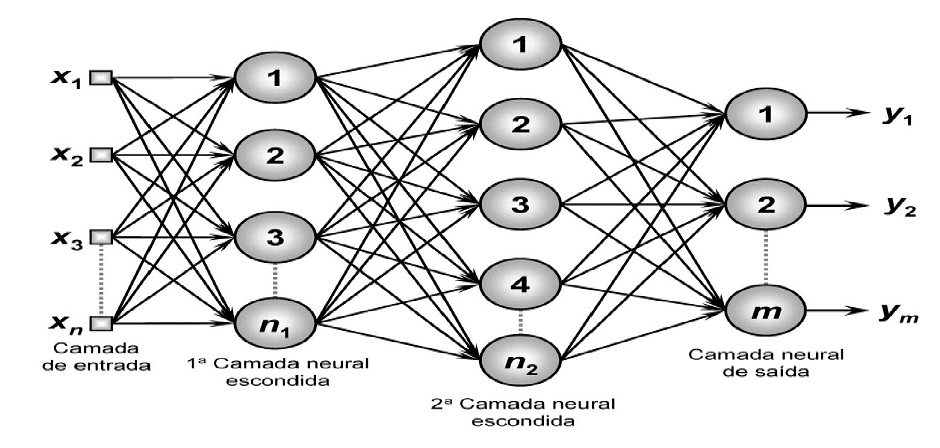
\includegraphics[scale=0.4]{pasta1_figuras/rna-Feedfoward.png}
    \caption{Neurônio Artificial}
\end{figure}

Em algumas arquiteturas é possível encontrar também interconexões das camadas no sentido da camada de saída em direção a camada de entrada. Tal arquitetura é denominada recorrente. Um exemplo dessa topologia pode ser observada na figura 2.3.
\begin{figure}[h]
	\centering
    \label{fig1}
    \vspace{3ex}%
	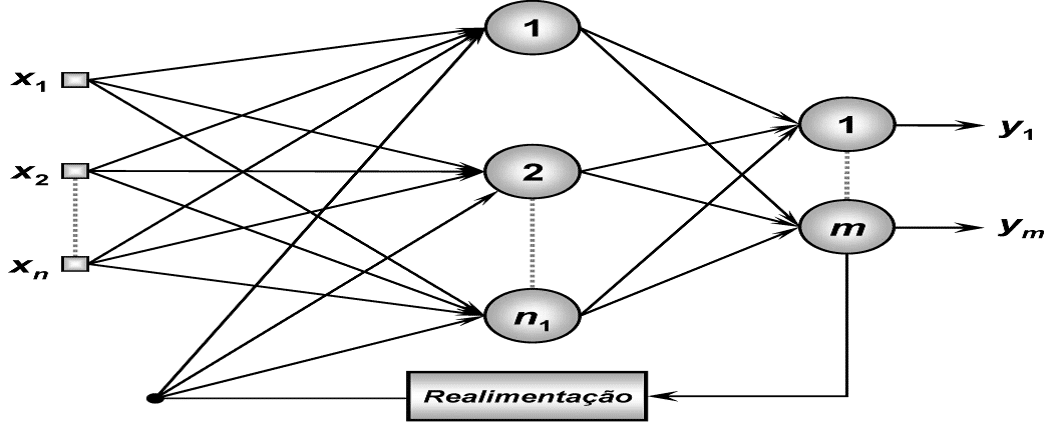
\includegraphics[scale=0.35]{pasta1_figuras/redes-recorrentes.png}
    \caption{Neurônio Artificial}
\end{figure}

Um dos conceitos fundamentais no projeto de redes neurais artificiais é o treinamento. O treinamento possui a função de ajustar os pesos da rede fazendo com que a mesma seja capaz de generalizar o aprendizado. Existem dois tipos de treinamento: Supervisionado e não supervisionado. O treinamento supervisionado é feito com o auxílio de um professor, ou seja, para um determinado conjunto de entradas existe uma saída conhecida e desejada. O aprendizado no treinamento não supervisionado será feito sem "professor" reconhecendo padrões, relações e regularidades sem conhecer as saídas.

Dentre os diversos algoritmos, destaca-se o backpropagation pela sua capacidade de resolver problemas não-linearmente separáveis. Este algoritmo só é aplicável em arquiteturas multicamadas e o seu processo de ajustes de pesos se baseia na retro propagação do erro. A perceptron multicamada é uma das arquiteturas que utiliza deste algoritmo de treino para generalizar suas soluções não-linearmente separáveis. Um exemplo de PMC pode ser visto a seguir:
\begin{figure}[h]
	\centering
    \label{fig1}
    \vspace{3ex}%
	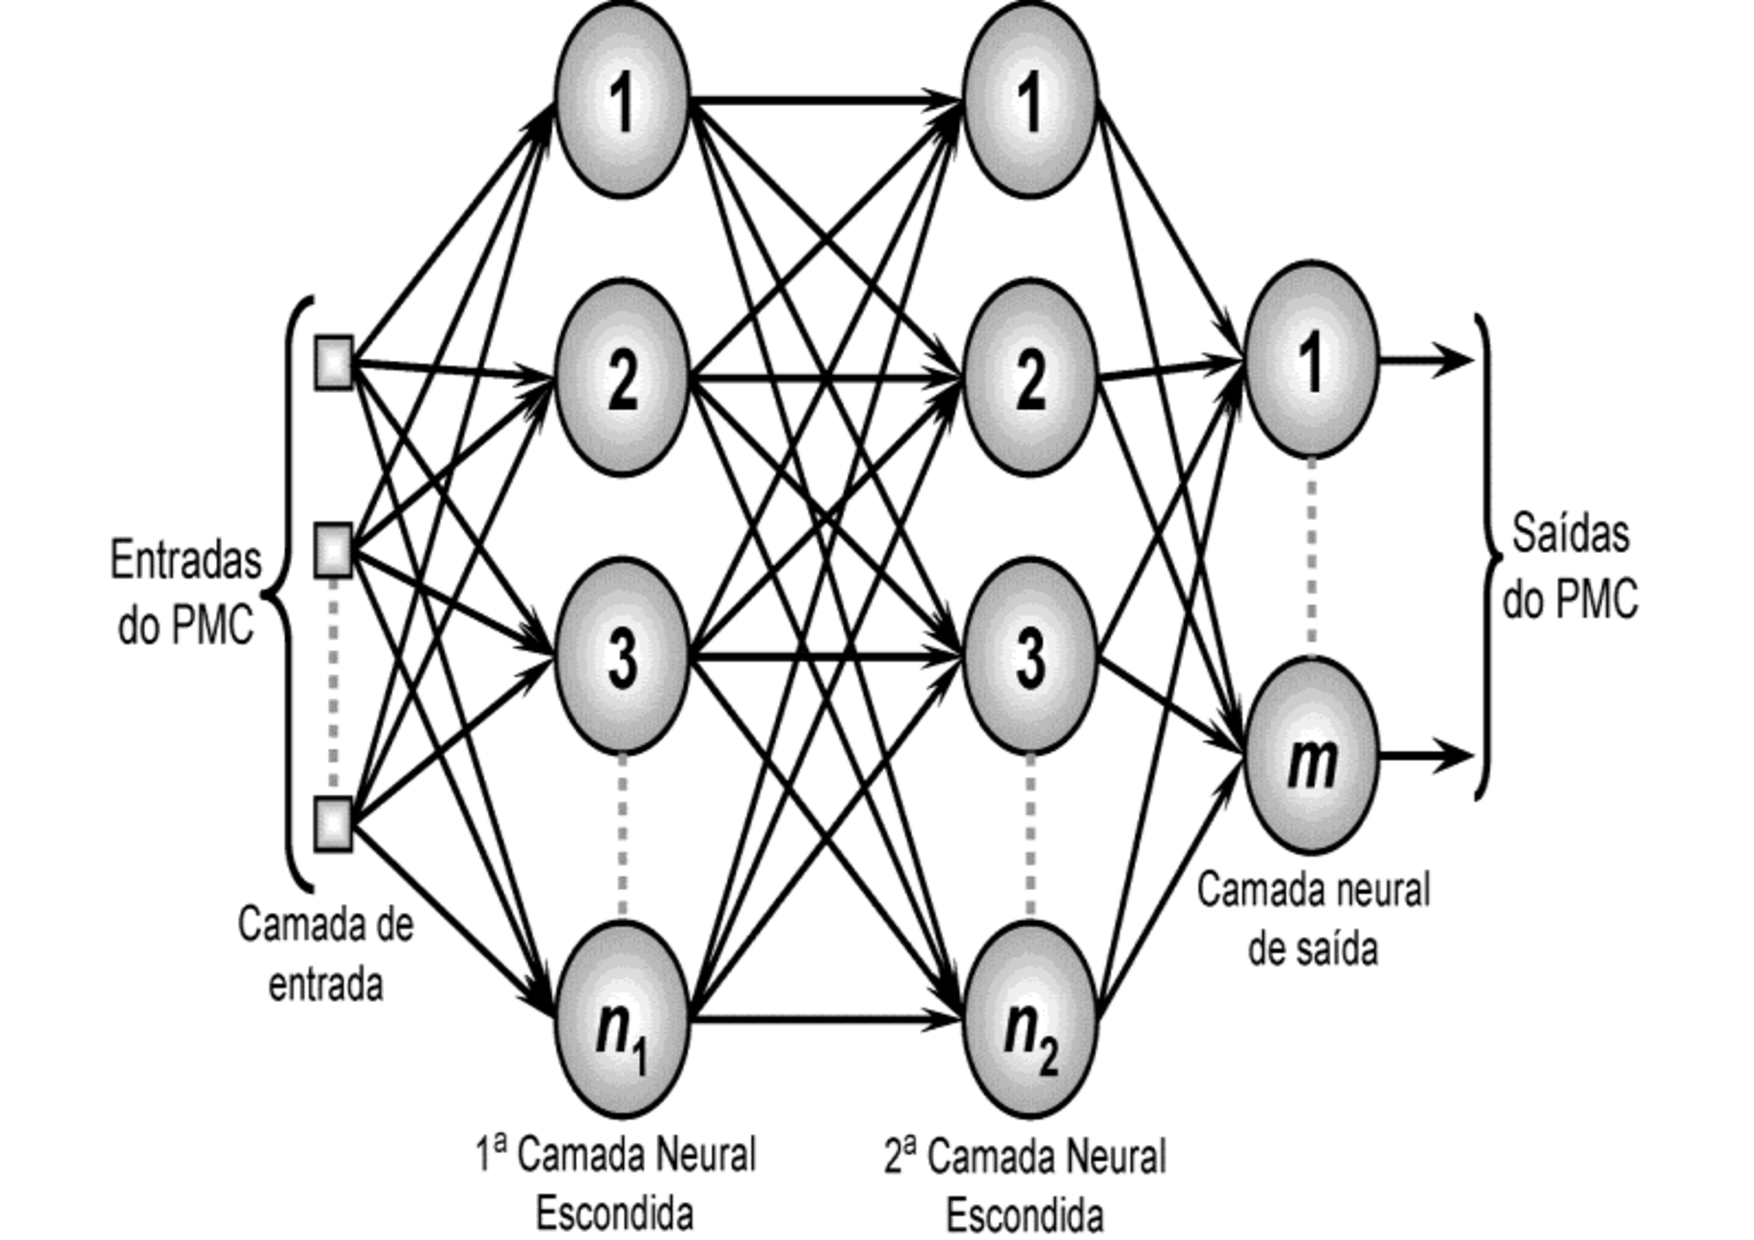
\includegraphics[scale=0.4]{pasta1_figuras/pmc.pdf}
    \caption{Neurônio Artificial}
\end{figure}

Overfitting e underfitting são classificações sobre a capacidade de generalização da rede. O overfitting ocorre quando a rede recebe treinamento demasiado das amostras do dataset, e no contrário, quando o treinamento é insuficiente ocorre o underfitting da capacidade de generalização. Para validar se uma rede neural já atende as especificações ótimas de generalização, ou seja, o ponto ótimo entre o overfitting e o underfitting. Alguns métodos de validação e testes já são utilizados no processo de treinamento de uma rede neural. Um muito conhecido é o método da validação cruzada, onde o dataset é dividido em 3 subconjuntos de amostras: Treino, validação e teste. O subconjunto do treino será o conjunto que treinará os pesos dos neurônios. Sob as amostras de validação serão calculados o erro até que se alcance a condição de parada. E por fim, o subconjunto de teste será usado para estipular os parametros da capacidade de generalização da rede. Na validação cruzada os subconjuntos de treino serão divididos em k partes iguais, onde cada k parte será o conjunto de validação durante uma certa quantidade de épocas de treino.
\subsection{Verificação}
Verificacao é um método utilizado para verificar a corretude de uma certa propriedade sob o funcionamento de um sistema. Tal técnica viza a validação e a confiabilidade de uma propriedade específica. Verificação se divide em dois tipos de abordagens: a verificação dedutiva e a verificação de modelos. No caso da primeira abordagem, a verificação permite a prova de propriedades temporais em sistemas com estados infinitos. Já na segunda abordagem, a verificação de modelos, do inglês Model Checking, trata do problema de testar de forma automática se um modelo de um determinado sistema atende a uma respectiva especificação, sendo que, por exemplo, tais especificações podem estar relacionadas com as propriedades de segurança e/ou de vivacidade do sistema em questão. Para solucionar este problema de forma algorítmica, é representado matematicamente o sistema e suas especificações utilizando métodos formais, como por exemplo, Lógica Proposicional e Lógica Temporal Linear, de tal forma que se possa verificar se uma dada fórmula é satisfeita dada uma determinada estrutura.

Ferramentas de software que executam a técnica de verificação automática são chamadas de verificadores. Esses se baseiam nas teorias da verificação de modelos, que possuem o objetivo de verificar de maneira rápida e eficiente propriedades de um código.

\subsection{GPU}
% Fim Capítulo